\documentclass{beamer}
\mode<presentation>
{
  \usetheme{Madrid}    
  \usecolortheme{beaver}
  \usefonttheme{serif}  
  \setbeamertemplate{navigation symbols}{}
  \setbeamertemplate{caption}[numbered]
} 

\usepackage[english]{babel}
\usepackage[utf8x]{inputenc}
\usepackage{xcolor}
\usepackage{listings}

\title[Intro to AI and ML]{Intro to AI and ML}
\author{Karthik Kanukollu, Praharsh Koppula}


\begin{document}

\begin{frame}
  \titlepage
  \begin{center}
      
  EE17BTECH11016, ME17BTECH11038
  \end{center}
\end{frame}

\section{Introduction}

\begin{frame}{Original Question}
    "Let O be the vertex and Q be any point on the parabola x$^2$ = 8y. If the point P divides the line segment OQ internally in the ratio 1:3, then the locus of P is:"
\end{frame}

\begin{frame}{Question in Matrix Form}
Let O be the vertex and Q be any point on the parabola \\ 
\begin{center}
    
\textbf{x$^T$}
\begin{bmatrix}
1 & 0 \\
0 & 0 \\
\end{bmatrix}
\textbf{x} + \textbf{x$^T$}
\begin{bmatrix}
0 \\
-8 \\
\end{bmatrix}=0.
\end{center}\\
If the point P divides the line segment OQ internally in the ratio 1:3, then find the locus of P.
\end{frame}
\begin{frame}{Solution}
	Let \textbf{P} = 
	\begin{bmatrix}
	x$_1$ \\
	y$_1$ \\
	\end{bmatrix} represent the point P. We need to find the locus of P.\\ 
	Given P divides the line segment OQ internally in the ratio 1:3. \\
	Thus, P = (1*Q + 3*O)/4.\\
	That is, P=Q/4, or Q=4*P\\
\end{frame}
\begin{frame}{Solution}
    	But we know that Q lies on the given parabola. Thus,\\
    	\begin{center}
    	    
    	16*\textbf{P$^T$}
    	\begin{bmatrix}
        1 & 0 \\
        0 & 0 \\
        \end{bmatrix}\textbf{P} + 4*\textbf{P$^T$}\begin{bmatrix}
0 \\
-8 \\
\end{bmatrix}=0.
        \end{center}\\
        Simplifying, we get:\\
        \begin{center}
    	\textbf{P$^T$}
    	\begin{bmatrix}
        1 & 0 \\
        0 & 0 \\
        \end{bmatrix}\textbf{P} + \textbf{P$^T$}\begin{bmatrix}
        0 \\
        -2 \\
        \end{bmatrix}=0.
        \end{center}
\end{frame}
\begin{frame}{Solution}
Replacing \textbf{P} with \textbf{x}, we get:\\
\begin{center}
        \textbf{x$^T$}
    	\begin{bmatrix}
        1 & 0 \\
        0 & 0 \\
        \end{bmatrix}\textbf{x} + \textbf{x$^T$}\begin{bmatrix}
        0 \\
        -2 \\
        \end{bmatrix}=0.
\end{center}\\
This is the locus of P.\\ Writing this in geometrical form, we get\\
\begin{center}
    x$^2$-2y=0.
\end{center}
\end{frame}
\begin{frame}{Plot}
In the plot, we can see that for different values of Q on the original parabola, the corresponding values of P lie on the calculated locus, thus confirming that our answer is correct.
\begin{center}
    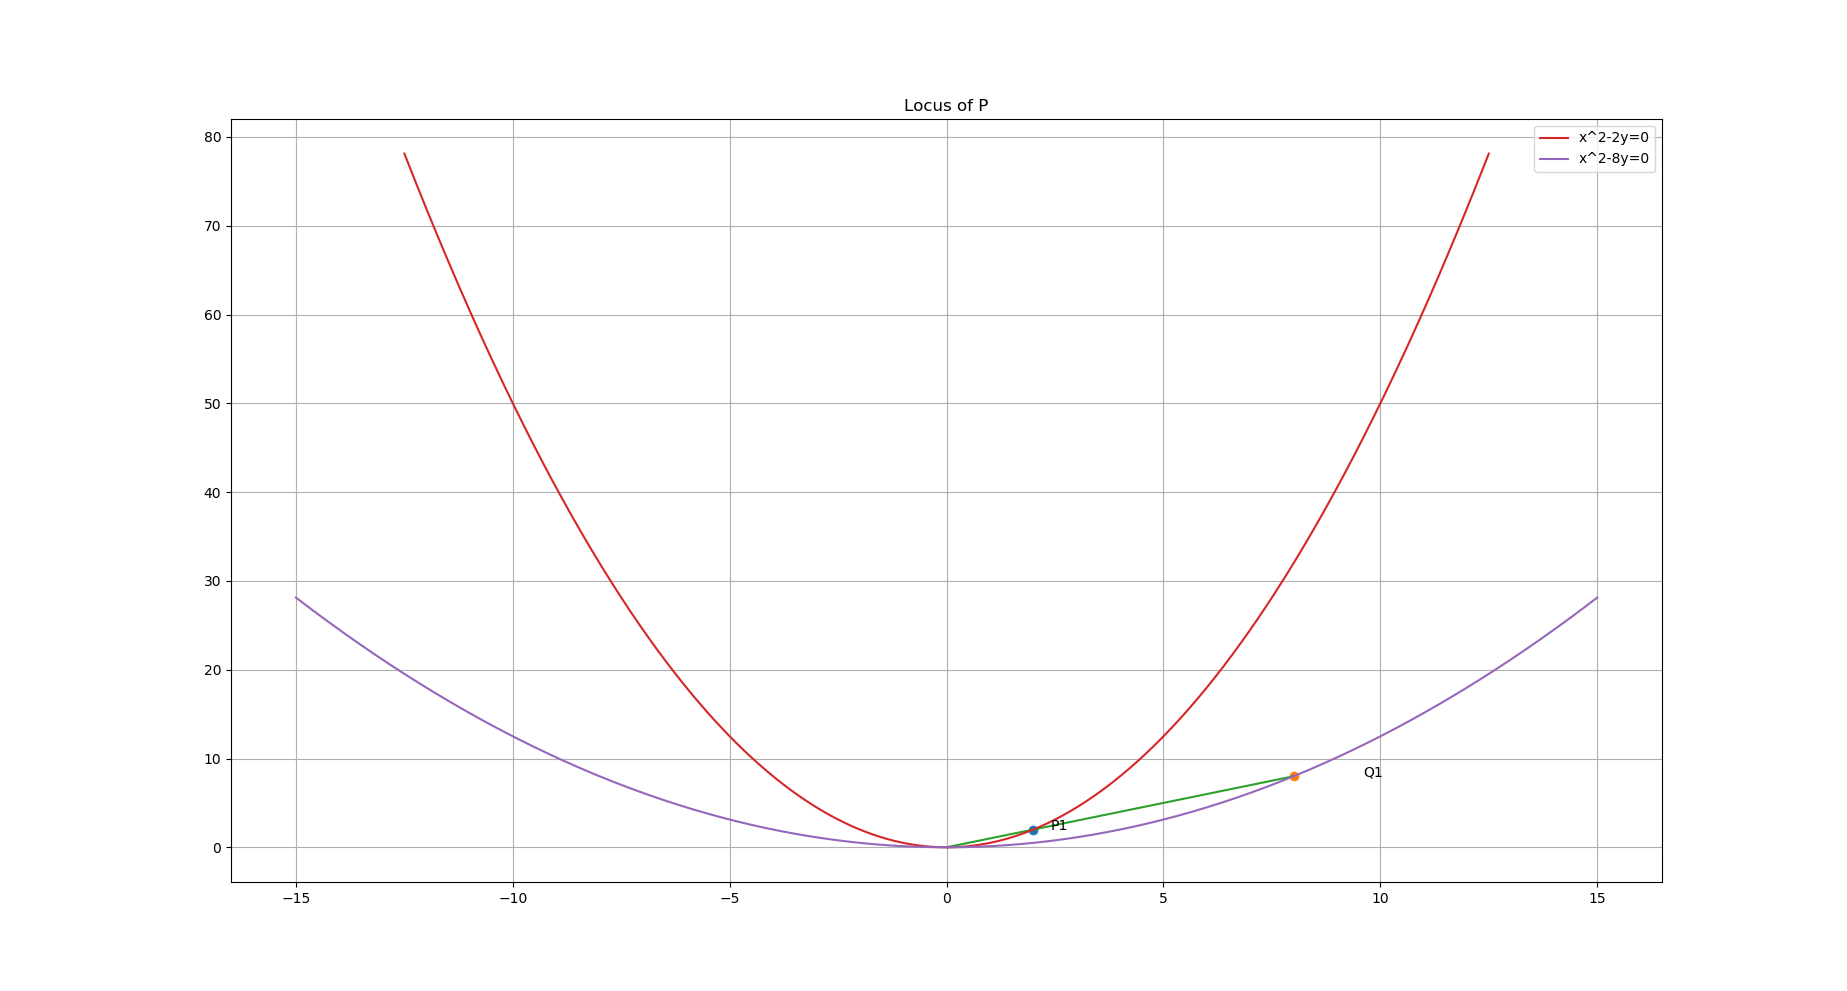
\includegraphics[scale = 0.2]{images/plot.png}
\end{center}
\end{frame}

\end{document}
